
\let\negmedspace\undefined
\let\negthickspace\undefined
\documentclass[journal,12pt,twocolumn]{IEEEtran}
%\documentclass[conference]{IEEEtran}
%\IEEEoverridecommandlockouts
% The preceding line is only needed to identify funding in the first footnote. If that is unneeded, please comment it out.
\usepackage{cite} %support for author-year citations 
\usepackage{amsmath,amssymb,amsfonts,amsthm}
\usepackage{algorithmic}
\usepackage{siunitx}
\usepackage{graphicx}
\usepackage{textcomp} %text symbols, such as the degree symbol,currency,etc
\usepackage{xcolor} %colored text and background colors
\usepackage{txfonts} %e fonts are designed to be used in mathematical expressions, and include characters such as the Greek alphabet, mathematical symbols, and operators
\usepackage{multirow}
%\usepackage{enumitem} %customizing the appearance of lists.
\usepackage{mathtools} %exp,eqn,subscript,superscript
\usepackage{gensymb} %scientific symbols
\usepackage[breaklinks=true]{hyperref} %This package provides support for hyperlinks within a LaTeX document, including clickable references and URLs. 
%The breaklinks=true option tells LaTeX to break long URLs that would otherwise extend beyond the right margin of the page. This can help to improve the readability of the document, as it avoids the need to scroll horizontally to read long URLs.

\usepackage{tkz-euclide} % loads  TikZ and tkz-base
%tools for drawing geometric figures in a LaTeX document, with a focus on Euclidean geometry

\usepackage{listings} %The listings package can be used to display code from various programming languages, including C, C++, Java, Python, and many others. It also provides options to customize the appearance of the listings, such as changing the font, background color, line numbers, and more.
%
%\usepackage{setspace}  %commands to control the line spacing
%\usepackage{gensymb} 
%\doublespacing
%\singlespacing
%\usepackage{graphicx} %to include graphics (images) 
%\usepackage{amssymb} %additional mathematical symbols and fonts \subset, \supset, \in, \exists, \forall, \not\equiv, etc.
% example for real numberset \mathbb{R} 
%\usepackage{relsize} %provides a simple way to adjust the font size of math mode symbols and text in a flexible way. It provides the \mathlarger and \mathsmaller commands to adjust the size of math mode symbols and the \larger and \smaller commands to adjust the size of text
%\usepackage[cmex10]{amsmath}
%\usepackage{amsthm}
%\interdisplaylinepenalty=2500
%\savesymbol{iint}
%\usepackage{txfonts}
%\restoresymbol{TXF}{iint}
%\usepackage{wasysym}
\usepackage{amsthm}
\usepackage{amsmath}
%\usepackage{iithtlc}
%\usepackage{mathrsfs}
%\usepackage{txfonts}
%\usepackage{stfloats}
%\usepackage{bm}
%\usepackage{cite}
%\usepackage{cases}
%\usepackage{subfig}
%\usepackage{xtab}
%\usepackage{longtable}
%\usepackage{multirow}
%\usepackage{algorithm}
%\usepackage{algpseudocode}
%\usepackage{enumitem}
%\usepackage{mathtools}
%\usepackage{tikz}
%\usepackage{circuitikz}
%\usepackage{verbatim}
%\usepackage{tfrupee}
%\usepackage{stmaryrd}
%\usetkzobj{all}
%    \usepackage{color}                                            %%
%    \usepackage{array}                                            %%
%    \usepackage{longtable}                                        %%
%    \usepackage{calc}                                             %%
%    \usepackage{multirow}                                         %%
%    \usepackage{hhline}                                           %%
%    \usepackage{ifthen}                                           %%
  %optionally (for landscape tables embedded in another document): %%
%    \usepackage{lscape}     
%\usepackage{multicol}
%\usepackage{chngcntr}
%\usepackage{enumerate}

%\usepackage{wasysym}
%\newcounter{MYtempeqncnt}
%\DeclareMathOperator*{\Res}{Res}
%\renewcommand{\baselinestretch}{2}
\renewcommand\thesection{\arabic{section}}
\renewcommand\thesubsection{\thesection.\arabic{subsection}}
\renewcommand\thesubsubsection{\thesubsection.\arabic{subsubsection}}

\renewcommand\thesectiondis{\arabic{section}}
\renewcommand\thesubsectiondis{\thesectiondis.\arabic{subsection}}
\renewcommand\thesubsubsectiondis{\thesubsectiondis.\arabic{subsubsection}}

% correct bad hyphenation here
\hyphenation{op-tical net-works semi-conduc-tor}
\def\inputGnumericTable{}                                 %%

\lstset{
%language=C,
frame=single, 
breaklines=true,
columns=fullflexible
}

\begin{document}
%


\newcommand{\BEQA}{\begin{eqnarray}}
\newcommand{\EEQA}{\end{eqnarray}}
\newcommand{\define}{\stackrel{\triangle}{=}}

\bibliographystyle{IEEEtran}
%\bibliographystyle{ieeetr}


\providecommand{\mbf}{\mathbf}
\providecommand{\pr}[1]{\ensuremath{\Pr\left(#1\right)}}
\providecommand{\qfunc}[1]{\ensuremath{Q\left(#1\right)}}
\providecommand{\sbrak}[1]{\ensuremath{{}\left[#1\right]}}
\providecommand{\lsbrak}[1]{\ensuremath{{}\left[#1\right.}}
\providecommand{\rsbrak}[1]{\ensuremath{{}\left.#1\right]}}
\providecommand{\brak}[1]{\ensuremath{\left(#1\right)}}
\providecommand{\lbrak}[1]{\ensuremath{\left(#1\right.}}
\providecommand{\rbrak}[1]{\ensuremath{\left.#1\right)}}
\providecommand{\cbrak}[1]{\ensuremath{\left\{#1\right\}}}
\providecommand{\lcbrak}[1]{\ensuremath{\left\{#1\right.}}
\providecommand{\rcbrak}[1]{\ensuremath{\left.#1\right\}}}
\theoremstyle{remark}
\newtheorem{rem}{Remark}
\newcommand{\sgn}{\mathop{\mathrm{sgn}}}
\providecommand{\abs}[1]{\left\vert#1\right\vert}
\providecommand{\res}[1]{\Res\displaylimits_{#1}} 
\providecommand{\norm}[1]{\left\lVert#1\right\rVert}
%\providecommand{\norm}[1]{\lVert#1\rVert}
\providecommand{\mtx}[1]{\mathbf{#1}}
\providecommand{\mean}[1]{E\left[ #1 \right]}
\providecommand{\fourier}{\overset{\mathcal{F}}{ \rightleftharpoons}}
%\providecommand{\hilbert}{\overset{\mathcal{H}}{ \rightleftharpoons}}
\providecommand{\system}{\overset{\mathcal{H}}{ \longleftrightarrow}}
	%\newcommand{\solution}[2]{\textbf{Solution:}{#1}}
\newcommand{\solution}{\noindent \textbf{Solution: }}
\newcommand{\cosec}{\,\text{cosec}\,}
\providecommand{\dec}[2]{\ensuremath{\overset{#1}{\underset{#2}{\gtrless}}}}
\newcommand{\myvec}[1]{\ensuremath{\begin{pmatrix}#1\end{pmatrix}}}
\newcommand{\mydet}[1]{\ensuremath{\begin{vmatrix}#1\end{vmatrix}}}
%\numberwithin{equation}{section}
%\numberwithin{equation}{subsection}
%\numberwithin{problem}{section}
%\numberwithin{definition}{section}
%\makeatletter
%\@addtoreset{figure}{problem}
%\makeatother

%\let\StandardTheFigure\thefigure
\let\vec\mathbf

\vspace{3cm}

\title{
Report on Hardwire Assignment\\Random Number Generation using Shift Registers\\AI1110 : Probability and Random Variables
}
\author{Tumarada Padmaja\\CS22BTECH11059}

% make the title area
\maketitle
%\newpage
\section{Components} 
\begin{table}[htbp]
\centering
%\caption{Components}
%%%%%%%%%%%%%%%%%%%%%%%%%%%%%%%%%%%%%%%%%%%%%%%%%%%%%%%%%%%%%%%%%%%%%%
%%                                                                  %%
%%  This is a LaTeX2e table fragment exported from Gnumeric.        %%
%%                                                                  %%
%%%%%%%%%%%%%%%%%%%%%%%%%%%%%%%%%%%%%%%%%%%%%%%%%%%%%%%%%%%%%%%%%%%%%%
\begin{tabular}{|c|c|c|}
\hline
Random Variable	&Value	&Event\\
\hline
\multirow{2}{*}X	&0	&not choosing black ball\\
\cline{2-3}
	&1	&choosing black ball\\
\hline
\end{tabular}

%\label{table:1}
\end{table}
\bigskip

\section{Description} 
1.Micro USB is used to get power supply and contains nodes such as Vbus and Gnd which refer to higher and lower voltage respectively. \\
2.Clock circuit is made using 555 timer IC, capacitors and resistor(higher one is chosen inorder to decrease the rate of change of the output ). It generates time delay in the circuit. It generates a square pulse which is checked using oscilloscope.\\
3.D Flipflops are connected to XOR gate each of 7474 IC contains two flipflops and hence toatl there are 4 flipflops. These overall create a binary output (output from each flipflop is either 0 or 1). XOR gate produces the randomness into the system .\\
4.Finally, the 4-bit output produced is decoded by the decoder ,7447 IC.\\
5.This decoder is connected to Seven Segment Display to get display of the random number produced. Decoder transforms output such that the appropriate segments on Seven Segment Display are illuminated in the range of 0 to 9.\\

\section{Block Diagram} 
\begin{figure}[h]
  \centering
  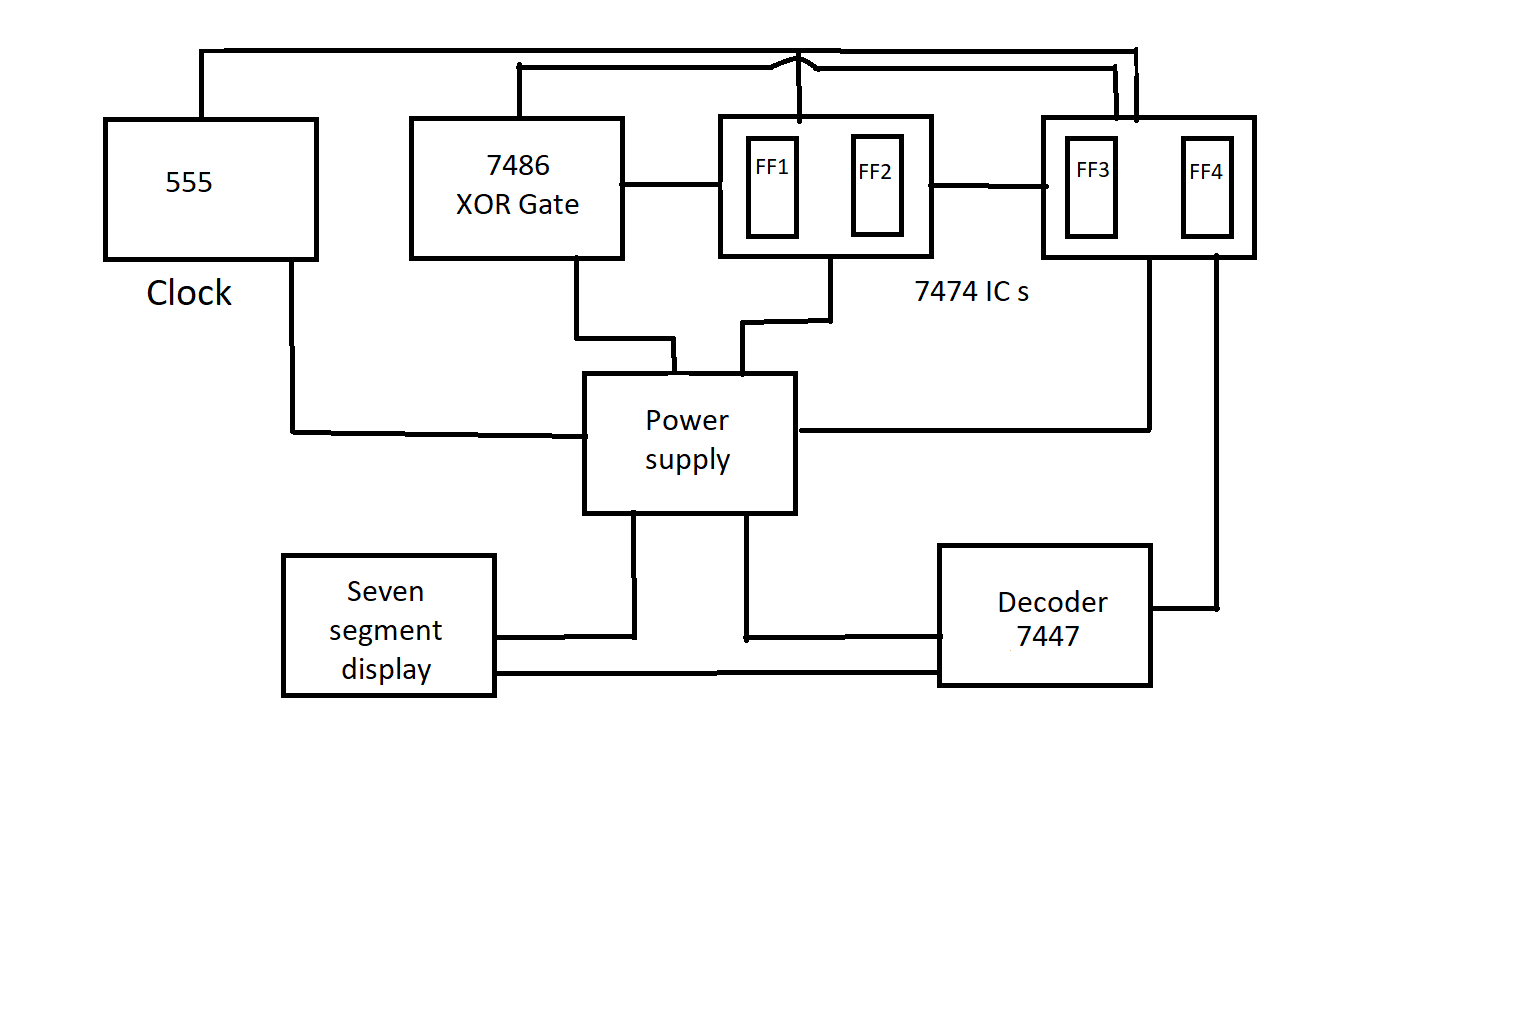
\includegraphics[width=0.5\textwidth]{blockdiagram_hardware.png}
\end{figure}


\begin{figure}[h]
\section{Observation} 
 
  \centering
  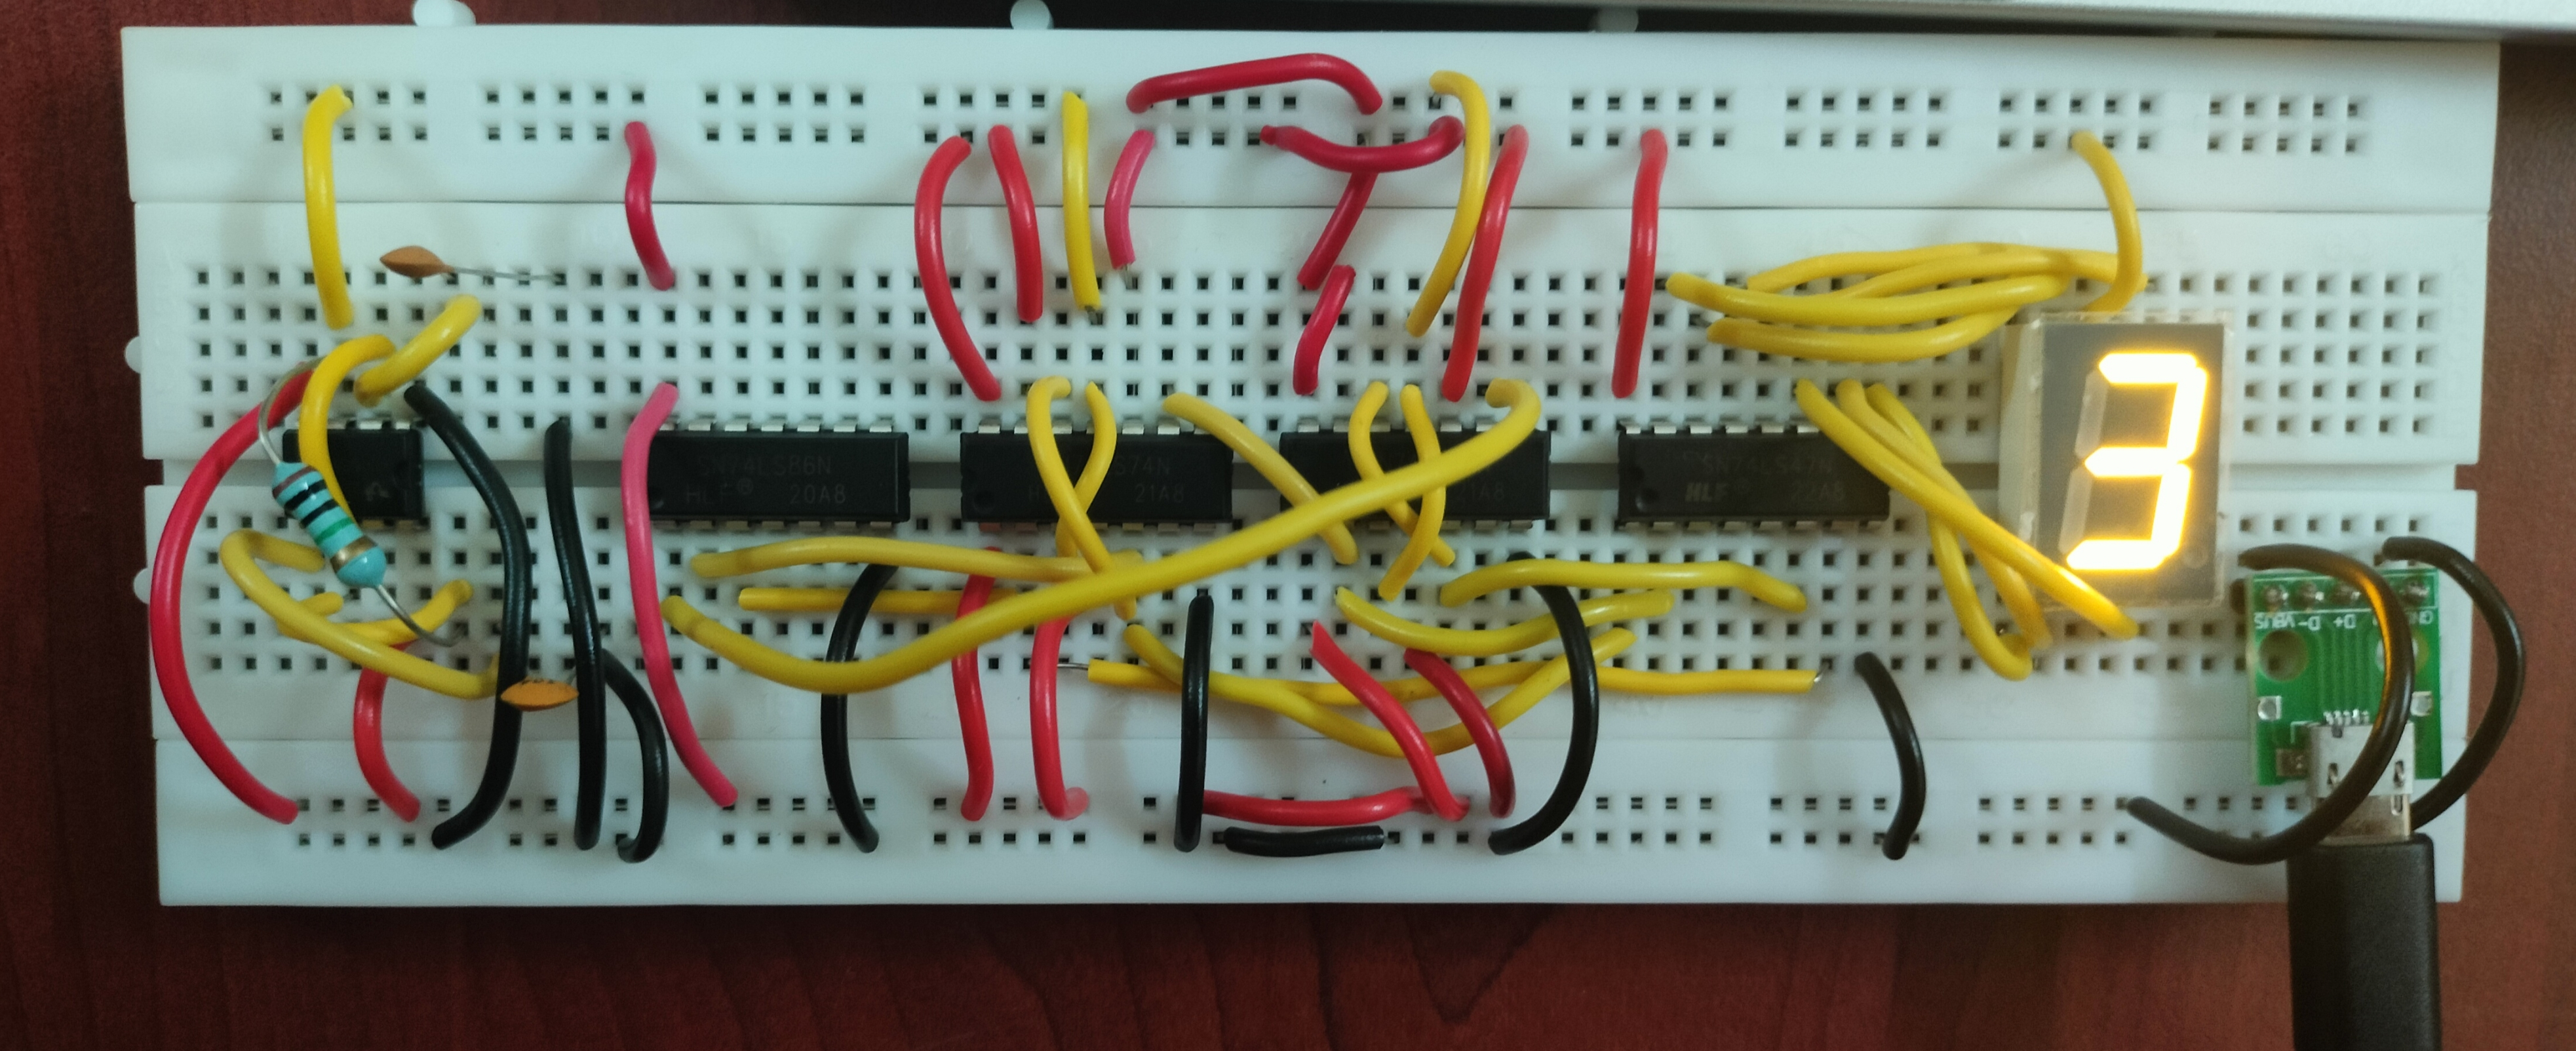
\includegraphics[width=0.3\textwidth]{images/ic1.jpg}
%  \caption{block diagram}
 % \label{fig:block diagram}

  \centering
  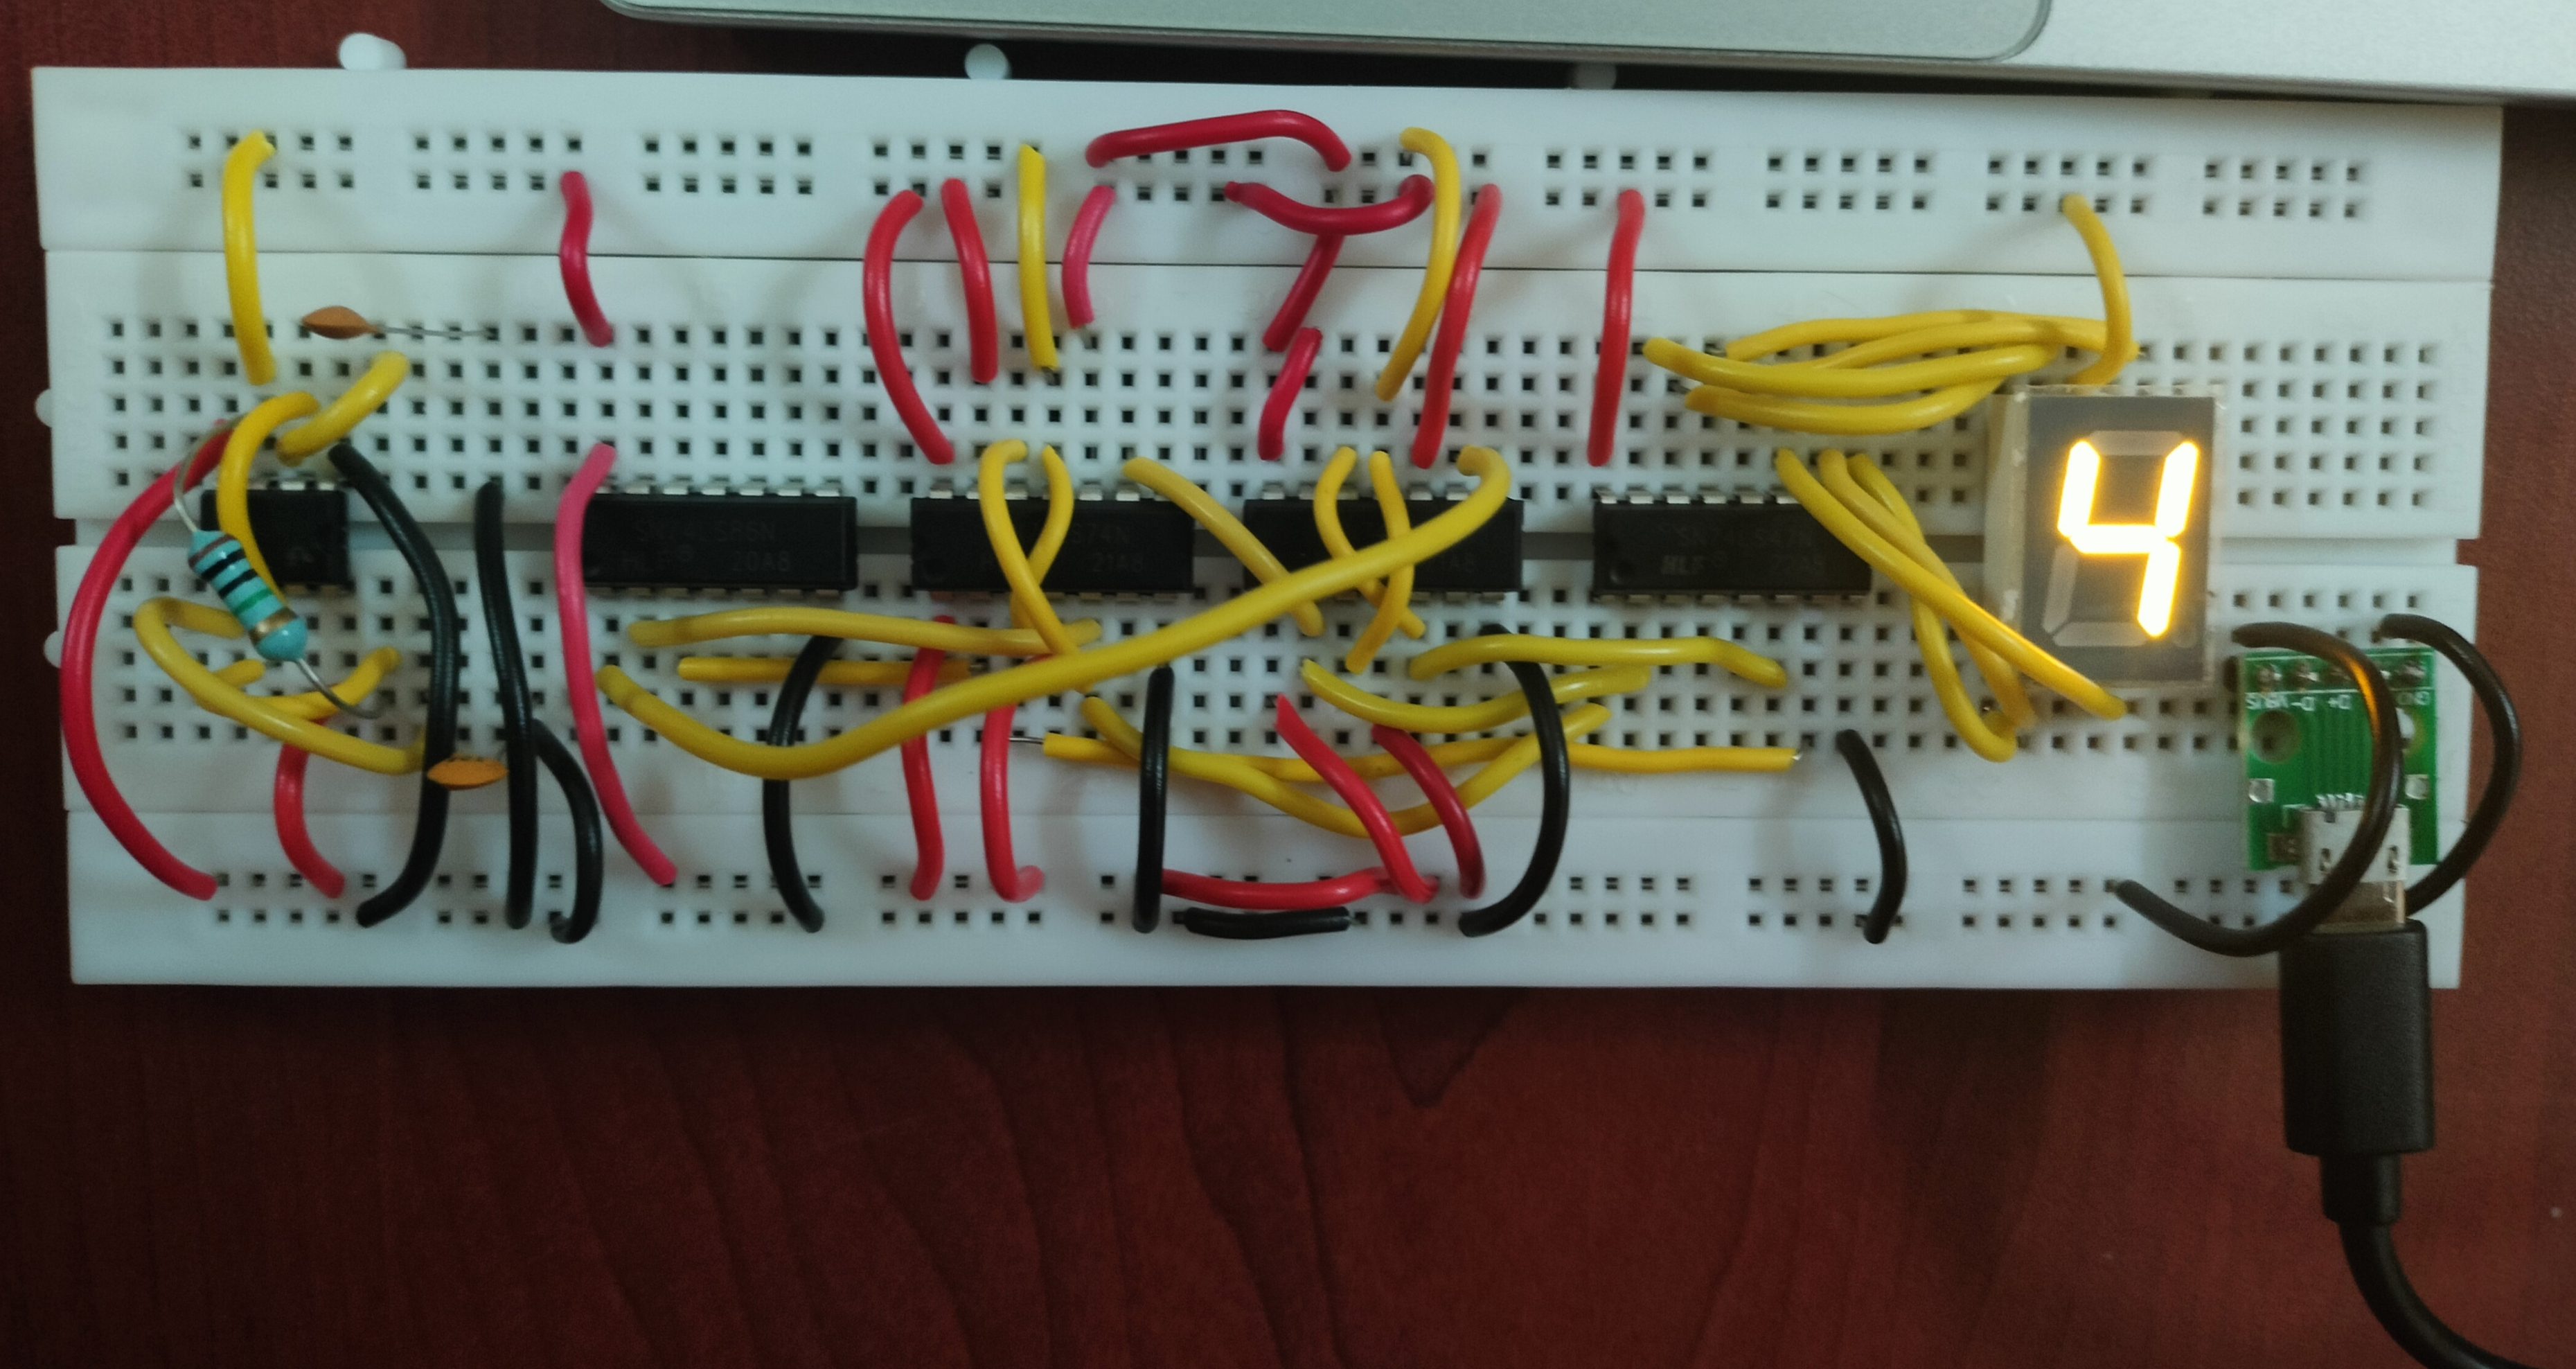
\includegraphics[width=0.3\textwidth]{images/ic2.jpg}
%  \caption{block diagram}
 % \label{fig:block diagram}

  \centering
  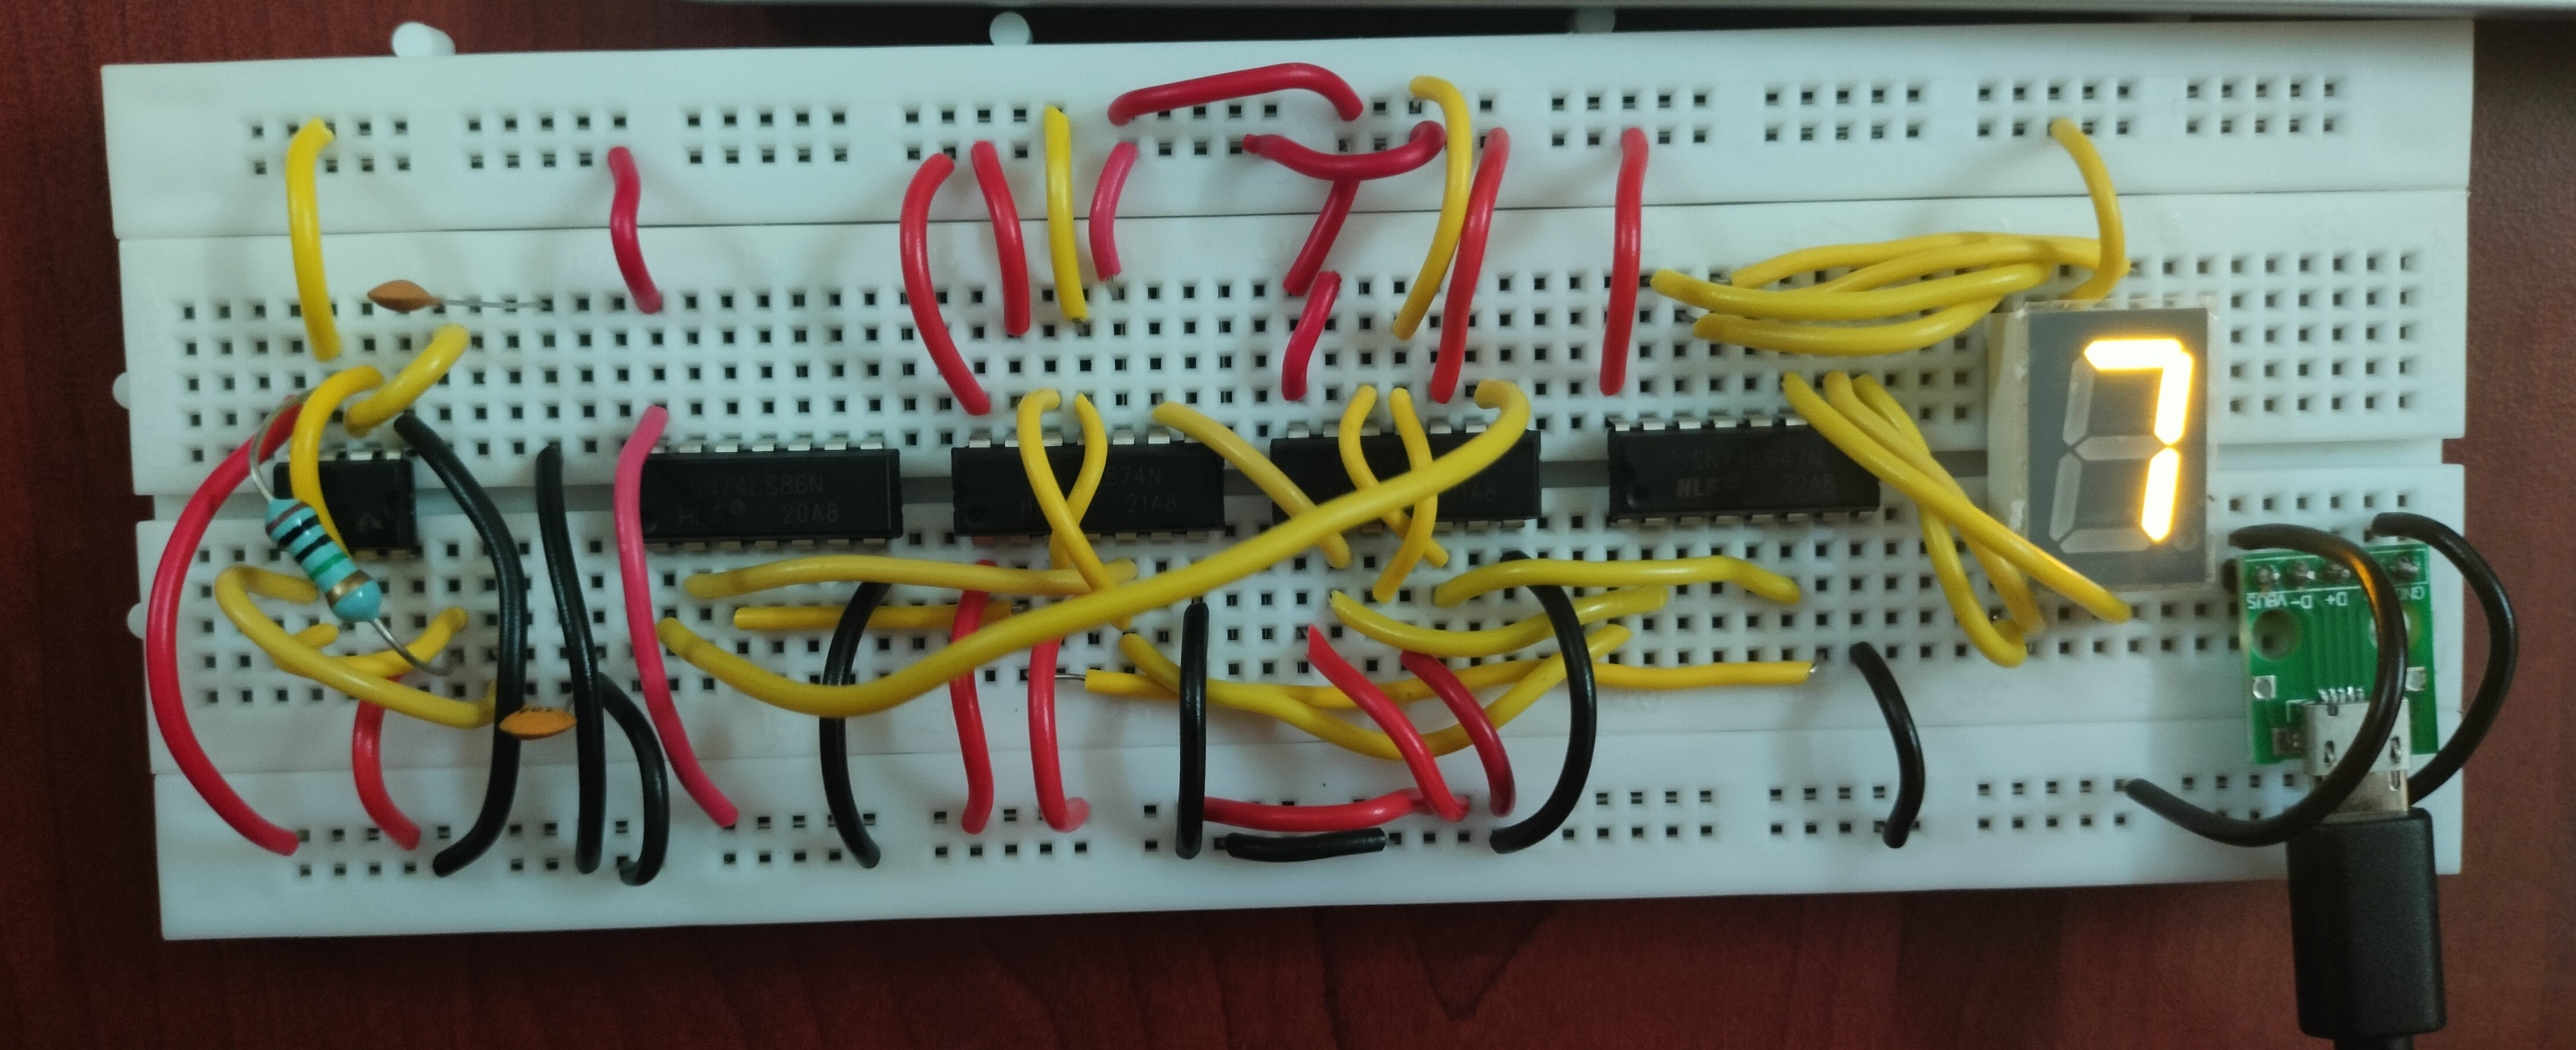
\includegraphics[width=0.3\textwidth]{images/ic3.jpg}
  %\caption{}
 % \label{fig:block diagram}
\end{figure}

 Random numbers are generated through the circuit where the time delay and frequency of change in numbers in display are influenced by the clock i.e capacitors and resistor in the circuit. Hence, the produced binary number by flipflops is decoded and displayed on the seven segment display as digits.
 
\end{document}


